% Copyright 2004 by Till Tantau <tantau@users.sourceforge.net>.
%
% In principle, this file can be redistributed and/or modified under
% the terms of the GNU Public License, version 2.
%
% However, this file is supposed to be a template to be modified
% for your own needs. For this reason, if you use this file as a
% template and not specifically distribute it as part of a another
% package/program, I grant the extra permission to freely copy and
% modify this file as you see fit and even to delete this copyright
% notice. 

\documentclass{beamer}

% There are many different themes available for Beamer. A comprehensive
% list with examples is given here:
% http://deic.uab.es/~iblanes/beamer_gallery/index_by_theme.html
% You can uncomment the themes below if you would like to use a different
% one:
%\usetheme{AnnArbor}
%\usetheme{Antibes}
%\usetheme{Bergen}
%\usetheme{Berkeley}
%\usetheme{Berlin}
%\usetheme{Boadilla}
%\usetheme{boxes}
%\usetheme{CambridgeUS}
%\usetheme{Copenhagen}
%\usetheme{Darmstadt}
%\usetheme{default}
%\usetheme{Frankfurt}
%\usetheme{Goettingen}
%\usetheme{Hannover}
%\usetheme{Ilmenau}
%\usetheme{JuanLesPins}
%\usetheme{Luebeck}
\usetheme{Madrid}
%\usetheme{Malmoe}
%\usetheme{Marburg}
%\usetheme{Montpellier}
%\usetheme{PaloAlto}
%\usetheme{Pittsburgh}
%\usetheme{Rochester}
%\usetheme{Singapore}
%\usetheme{Szeged}
%\usetheme{Warsaw}
\newcommand*{\argmin}{\operatornamewithlimits{argmin}\limits}
\newcommand*{\argmax}{\operatornamewithlimits{argmax}\limits}

\title{Final Project: Crowd-sourcing}

% A subtitle is optional and this may be deleted
\subtitle{IE 598 Inference in Graphical Models}

\author{Kiran Koshy .~Thekumparampil\inst{1} \and Pavankumar Reddy.~Muddireddy\inst{1}}
% - Give the names in the same order as the appear in the paper.
% - Use the \inst{?} command only if the authors have different
%   affiliation.

\institute[Universities of Illinois] % (optional, but mostly needed)
{
  \inst{1}%
  Department of Electrical and Computer Engineering\\
  University of Illinois}
% - Use the \inst command only if there are several affiliations.
% - Keep it simple, no one is interested in your street address.

\date{Inference in Graphical Models\\
        Final Project Presentation, 2015}
% - Either use conference name or its abbreviation.
% - Not really informative to the audience, more for people (including
%   yourself) who are reading the slides online

\subject{Graphical Models}
% This is only inserted into the PDF information catalog. Can be left
% out. 

% If you have a file called "university-logo-filename.xxx", where xxx
% is a graphic format that can be processed by latex or pdflatex,
% resp., then you can add a logo as follows:

% \pgfdeclareimage[height=0.5cm]{university-logo}{university-logo-filename}
% \logo{\pgfuseimage{university-logo}}

% Delete this, if you do not want the table of contents to pop up at
% the beginning of each subsection:
\AtBeginSubsection[]
{
  \begin{frame}<beamer>{Outline}
    \tableofcontents[currentsection,currentsubsection]
  \end{frame}
}

% Let's get started
\begin{document}

\begin{frame}
  \titlepage
\end{frame}

\begin{frame}{Outline}
  \tableofcontents
  % You might wish to add the option [pausesections]
\end{frame}

% Section and subsections will appear in the presentation overview
% and table of contents.
\section{Model}

\subsection{Graphical Model for crowdsourcing}

\begin{frame}{Likelihood of tasks labels and reliability parameters}
  \begin{itemize}
  \item {
    The joint likelihood for tasks labels($i$) denoted by $t_i$ and reliability parameters for worker($j$) denoted by $p_j$ given responses $A_{ij}$ (to task $i$ by worker $j$) is denoted by $\mu(t,p|A)$
  }
  \item {
    $$\mu(t,p|A) \propto \mu(t,p,A) \propto \mu(A|t,p)\mu(t)\mu(p)$$
    $$\mu(t,p|A) = \frac{1}{Z}\prod_{i\in [n]}{F'(t_i)}\prod_{j\in [m]}{F(p_j)}\prod_{(i,j)\in E}(\psi_{ij}(A_{ij},p_j,t_j))$$
    where, $\psi_{ij}(A_{ij}, p_j, t_j) = \mathbb{I}(t_i=A_{ij})p_j + \mathbb{I}(t_i=-A_{ij})(1-p_j)$
  }
  \item {
  Here $F'(t_i)$ is the bernoulli (0.75) prior of task labels and $F(p_j)$ is the beta distribution with $\alpha = 6$ and $\beta = 2$
  }
  \end{itemize}
\end{frame}

\subsection{Model for Expectation Maximization}

\begin{frame}{Likelihood of tasks labels and reliability parameters}
  \begin{itemize}
  \item {
    The likelihood for tasks labels given responses $A_{ij}$ using reliability parameters for workers as parameters for the EM is denoted by 
    $\mu_p(t|A)$
  }
  \item {
    $$\mu_p(t|A) = \frac{1}{Z}\prod_{i\in [n]}{F'(t_i)}\prod_{(i,j)\in E}(\psi_{p_j}(A_{ij},t_j))$$
    where, $\psi_{p_j}(A_{ij}, t_j) = \mathbb{I}(t_i=A_{ij})p_j + \mathbb{I}(t_i=-A_{ij})(1-p_j)$
  }
  \end{itemize}
\end{frame}

\iffalse
% You can reveal the parts of a slide one at a time
% with the \pause command:
\begin{frame}{Likelihood of tasks with reliabilities as parameters}
  \begin{itemize}
  \item {
    First item.
    \pause % The slide will pause after showing the first item
  }
  \item {   
    Second item.
  }
  % You can also specify when the content should appear
  % by using <n->:
  \item<3-> {
    Third item.
  }
  \item<4-> {
    Fourth item.
  }
  % or you can use the \uncover command to reveal general
  % content (not just \items):
  \item<5-> {
    Fifth item. \uncover<6->{Extra text in the fifth item.}
  }
  \end{itemize}
\end{frame}
\fi




\section{Belief Propagation update Equations}
\subsection{Message passing algorithm}

\begin{frame}{Quantization of beta distribution}
    \begin{itemize}
    \item {
    Since, the beta distribution is continuous and hence, the message passing would involve passing a continuous distribution from each worker to task and also integration at each task message to worker, the distribution is quantized to discrete points.
    }
    \item {
    In effect, this would be like having probability of each $p_k$ belonging to an interval and the sum would be equivalent to approximate numerical integration.
    }
    \end{itemize}
\end{frame}

\begin{frame}{Message passing algorithm}
  \begin{itemize}
  \item {
  From the joint distribution earlier the messages from different kinds of nodes in the graph are,
  }
  \item {
  Messages from worker to task,
  $$\nu_{j\rightarrow i}\propto\prod_{k\in \partial j\setminus i}\sum_{t_k}F'(t_k)\psi_{kj}(t_k, p_j)\nu_{k\rightarrow j}(t_k)$$
  }
  \item {
  Messages from task to workers,
  $$\nu_{i\rightarrow j}\propto\prod_{k\in \partial i\setminus j}\sum_{p_k}F(p_k)\psi_{kj}(t_i, p_k)\nu_{k\rightarrow i}(p_k)$$
  }
  \end{itemize}
\end{frame}





\section{Expectation Maximization}
\subsection{Objective}

\begin{frame}{Objective in EM}
    \begin{itemize}
    \item {
    The EM is formulated with $p_j$'s as parameters, again to handle the continuous nature of the distribution.
    }
    \item {
    Hence, the objective would to find the parameters that would maximize the likelihood,
    }
    \item {
    $$p* = \argmax_p\mu_p(A) = \argmax_p\sum_{t\in\{-1,+1\}^n}\mu_p(t,A)$$
    where $\mu_p(t,A) = \frac{1}{Z}\prod_{i\in [n]}{F'(t_i)}\prod_{(i,j)\in E}(\psi_{p_j}(A_{ij},t_j))$
    }
    \end{itemize}
\end{frame}

\begin{frame}{Message passing algorithm}
  \begin{itemize}
  \item {
  $q_i(.)$ initialized to fraction of positive and negative responses respectively for $i$ (majority voting).
  $$p_j = \frac{\sum_{i\in \partial j}q(A_{ij})}{|\partial j|}$$
  }
  \item {
  Update equations:
  $$q_i(t_i) \leftarrow \frac{F'(t_i)\prod_{j\in \partial i} \mu_{p_j}(A_{ij}|t_i)}{\sum_{t'_i\in {-1,+1}}F'(t'_i)\prod_{j\in \partial i} \mu_{p_j}(A_{ij}|t'_i)}$$
  $$p_j \leftarrow \frac{\sum_{i\in \partial j}q(A_{ij})}{|\partial j|}$$
  }
  \end{itemize}
\end{frame}



\subsection{Design of the task Assignment}

\begin{frame}{Design of the task Assignment}
    \begin{itemize}
    \item {
    Given a number of tasks and workers with $l$ and $r$ parameters, Erd\H{o}s-R\'enyi is not used, rather a random $(l, r)$ graph is generated by taking $nl$ half edges and $mr$ half edges and connecting a random permutation of them. This ensures that the degree distribution is uniform  across both tasks and workers instead of bernoulli as in Erd\H{o}s-R\'enyi graph.
    }
    \end{itemize}
\end{frame}



\subsection{Results with EM}

\begin{frame}{Results with plain EM}
    \begin{itemize}
    \item {
    The plot of error with number of workers,
    \begin{figure}[h!]
   %\caption{A picture of a gull.}
   \centering
     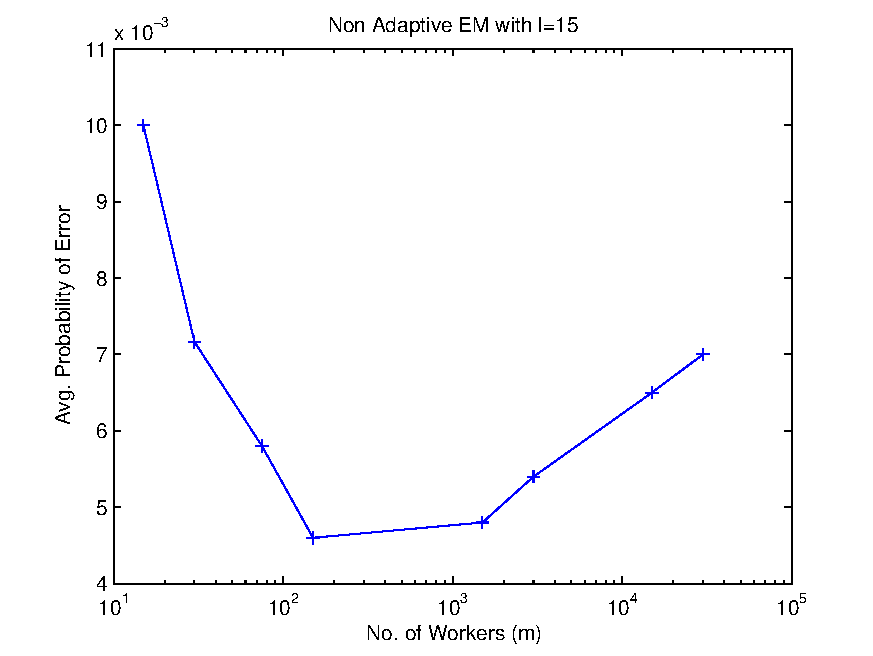
\includegraphics[width=0.75\textwidth]{worker_error.pdf}
\end{figure}
    }
    \end{itemize}
\end{frame}

\begin{frame}{Results with plain EM}
    \begin{itemize}
    \item {
    The plot of quality with number of workers,
    \begin{figure}[h!]
   %\caption{A picture of a gull.}
   \centering
     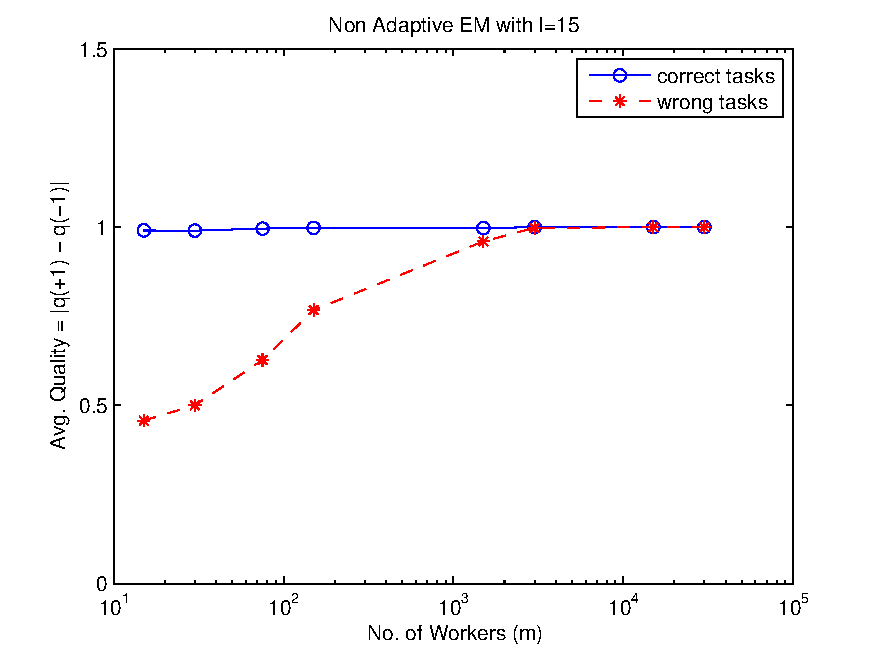
\includegraphics[width=0.75\textwidth]{quality_diff2.pdf}
\end{figure}
    }
    \end{itemize}
\end{frame}


\subsection{Observations from plain EM}

\begin{frame}{Observations with plain EM}
    \begin{itemize}
    \item {
    The quality of a task estimate is defined as $|q(+1) - q(-1)|$, which indicates the amount of uncertainty in the prediction of a task label. So, low quality indicates, very high uncertainty.
    }
    \item {
    From the plot of quality distribution for misclassified tasks, it can be seen that the quality is a very good metric for classification error for a given task.
    }
    \item {
    So, any adaptation done could use quality of task estimates to assign more workers for a given tasks.
    }
    \end{itemize}
\end{frame}


\begin{frame}{Observations with plain EM}
    \begin{itemize}
    \item {
    Additionally, one could define similar quality for the workers with $|2p_j-1|$, which indicates how uncertain the worker was in giving the response for a given task.
    }
    \item {
    One could remove low quality workers. But its been observed that losing budget, even low quality, was very detrimental to the estimates. So, the task estimates were very sensitive to the their fanout.
    }
    \end{itemize}
\end{frame}




\begin{frame}{Adaptive EM Algorithm}
    \begin{itemize}
    \item{
    Our adaptive algorithm progressively adds half of budget left at each iteration.
    }
    \item{
    After the each run of EM we take the bottom half of the tasks ranked by quality plus bottom hundredth of the tasks ranked by degree and add half of the budget left to these tasks by connecting them to new workers.}
    \item{
    For initialization estimates of tasks and workers are copied from the previous iterations}
    \item{
    This is done till budget is exhausted.}
    \end{itemize}
\end{frame}


\begin{frame}{Observations in adapted EM}
    \begin{itemize}
    \item {
    As seen in the earlier plain EM, keeping the number of workers in the order of number of tasks was non-ideal. This was again observed in adapted EM.
    }
    \item {
    Could be because $p_j$ estimate needs a large $r$ which intern implies a small $m$ for a given budget $n\times l$.
    }
    \item {
    Ideal estimates when $m = l$ or $m = 2l$.
    }
    \item {
    The adapted EM with more workers just for low quality workers was not giving some outliers with good quality but an incorrect estimate of label. Its been seen that degree of such nodes was low. (We start out with uniform degree but it changes as more wokers are added to some of the tasks). So, low degree tasks are also provided with more workers.
    }
    \end{itemize}
\end{frame}




\begin{frame}{Final Results in adapted EM}
    \begin{itemize}
    \item {
    The plot of error with $l$,
    \begin{figure}[h!]
   %\caption{A picture of a gull.}
   \centering
     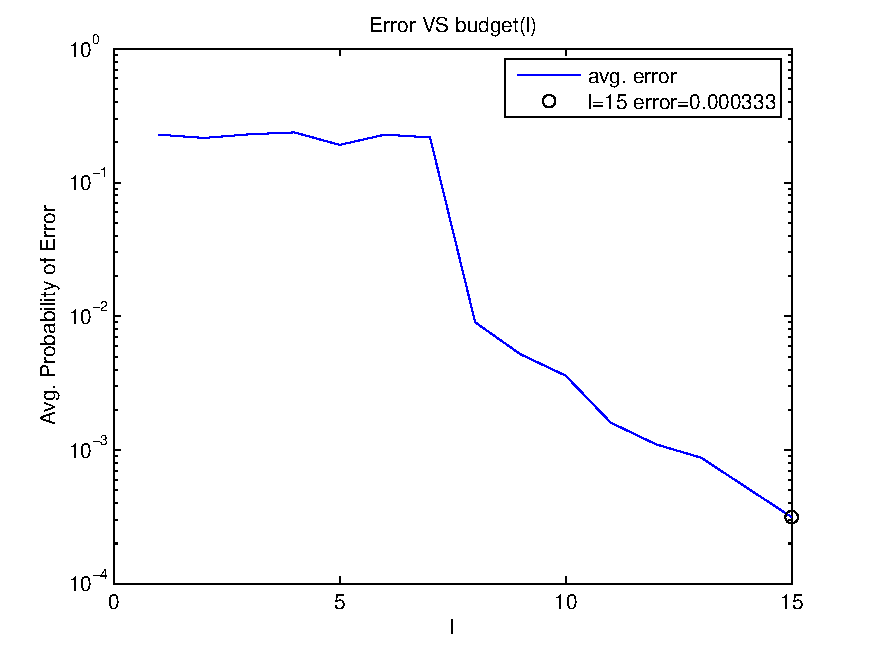
\includegraphics[width=0.75\textwidth]{avg_error1.pdf}
\end{figure}
    }
    \end{itemize}
\end{frame}



\begin{frame}{Final Results in adapted EM}
    \begin{itemize}
    \item {
    The plot of error with $l$, The final error is $3.33\times 10^{-4}$ for $m = l$ and $2\times 10^{-4}$ for $m = 2l$
    \begin{figure}[h!]
   %\caption{A picture of a gull.}
   \centering
     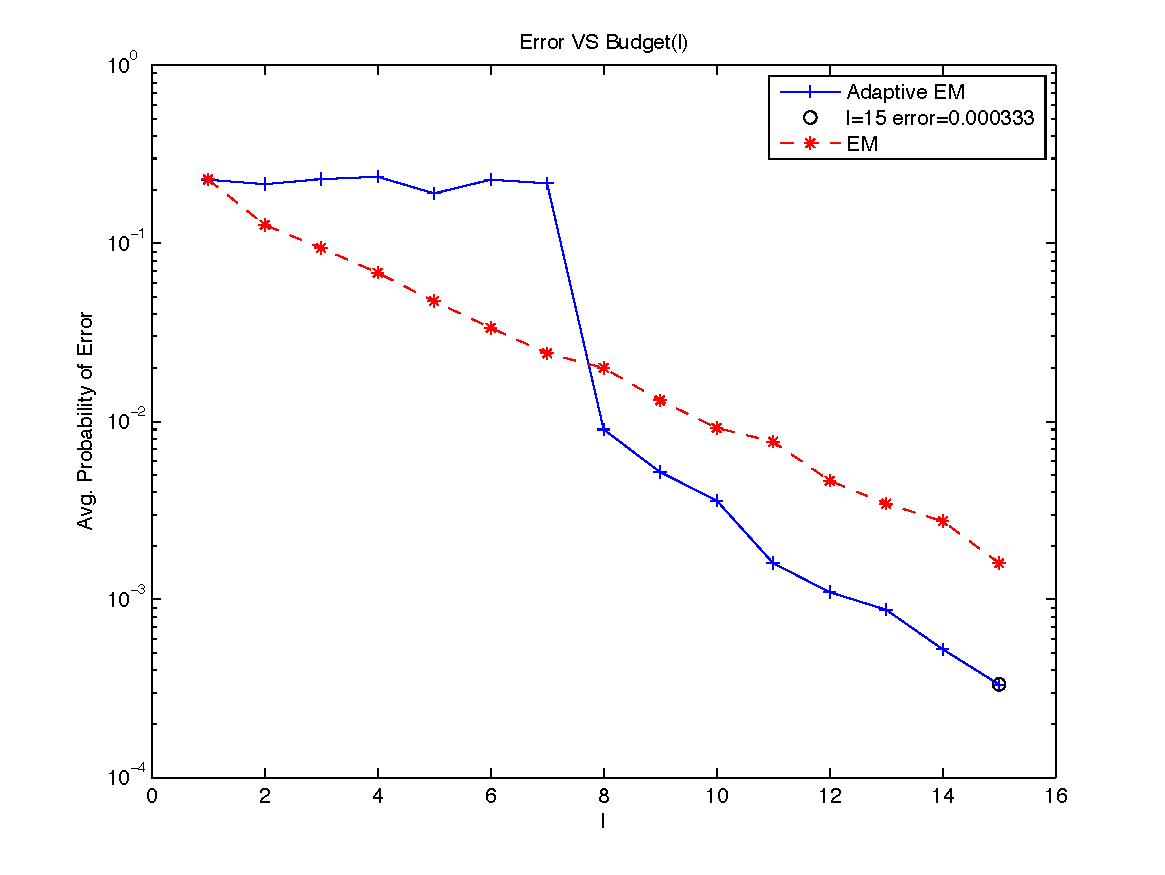
\includegraphics[width=0.75\textwidth]{avg_error2.pdf}
\end{figure}
    }
    \end{itemize}
\end{frame}




\iffalse
\section{Second Main Section}

\subsection{Another Subsection}

\begin{frame}{Blocks}
\begin{block}{Block Title}
You can also highlight sections of your presentation in a block, with it's own title
\end{block}
\begin{theorem}
There are separate environments for theorems, examples, definitions and proofs.
\end{theorem}
\begin{example}
Here is an example of an example block.
\end{example}
\end{frame}

% Placing a * after \section means it will not show in the
% outline or table of contents.
\section*{Summary}

\begin{frame}{Summary}
  \begin{itemize}
  \item
    The \alert{first main message} of your talk in one or two lines.
  \item
    The \alert{second main message} of your talk in one or two lines.
  \item
    Perhaps a \alert{third message}, but not more than that.
  \end{itemize}
  
  \begin{itemize}
  \item
    Outlook
    \begin{itemize}
    \item
      Something you haven't solved.
    \item
      Something else you haven't solved.
    \end{itemize}
  \end{itemize}
\end{frame}



% All of the following is optional and typically not needed. 
\appendix
\section<presentation>*{\appendixname}
\subsection<presentation>*{For Further Reading}

\begin{frame}[allowframebreaks]
  \frametitle<presentation>{For Further Reading}
    
  \begin{thebibliography}{10}
    
  \beamertemplatebookbibitems
  % Start with overview books.

  \bibitem{Author1990}
    A.~Author.
    \newblock {\em Handbook of Everything}.
    \newblock Some Press, 1990.
 
    
  \beamertemplatearticlebibitems
  % Followed by interesting articles. Keep the list short. 

  \bibitem{Someone2000}
    S.~Someone.
    \newblock On this and that.
    \newblock {\em Journal of This and That}, 2(1):50--100,
    2000.
  \end{thebibliography}
\end{frame}
\fi

\end{document}


